% !TeX spellcheck = en_US
\addscenariosection[subsection]{1}{Castle Campaign $-$ The Queen's Gambit}{2. Sicilian Dragon}{\images/catherine.png}

\begin{multicols*}{2}

\textbf{Author:} Tyson Heckert

\textbf{Source:} \href{https://travelledtales.com}{travelledtales.com}

\textit{Convinced that the only way to save Steadwick is to attack Vhidhax, Catherine powers her small force ahead.
Following the Archangels to a distant, inhospitable land, she must now navigate her way through.}

\subsection*{\MakeUppercase{Scenario length}}

This Scenario plays out over 11 Rounds.

\subsection*{\MakeUppercase{Player setup}}

\textbf{Faction:} Castle

\textbf{Faction Hero:} The same Hero as Scenario 1

\textbf{Starting Resources:} The resources you ended with in Scenario 1

\textbf{Starting Income:} 10 \svg{gold}, 0 \svg{building_materials}, 0 \svg{valuables}

\textbf{Starting Units:} The army you ended with in Scenario 1

\textbf{Town Buildings:} None

\textbf{Bonus:} Begin the Scenario at Hero Level 2, but do not take new Ability Cards.

\subsection*{\MakeUppercase{AI Hero setup}}

\textbf{Faction:} Necropolis

\textbf{Enemy Army:} A Pack of Skeletons, a Pack of Zombies, a Pack of Liches, a Few Dread Knights, a Few Ghost Dragons

\textbf{Enemy Deck:} 3 × Might Cards, 3 × Magic Cards, 1 × Skill Card

\textbf{Enemy Spells:} 2 × Lightning Bolt, 1 × Curse

\textbf{Enemy Skills:} Cloak of the Undead King IV and VI, the enemy will play whichever it can

\textbf{Neutral Enemy Deck:} 4 × Might Cards

\subsection*{\MakeUppercase{Map setup}}

Take the following Map Tiles and arrange them as shown in the Scenario map layout:

\textbf{1 × Starting (I) Map Tile}
\begin{itemize}
    \item 1 × Necropolis (S1)
\end{itemize}

\textbf{3 × Far (II--III) Map Tile}
\begin{itemize}
    \item 3 × random Tiles from Necropolis or Dungeon (F1, F2, F4, F5, F7, F8)
\end{itemize}

\textbf{4 × Near (IV--V) Map Tile}
\begin{itemize}
    \item 2 × Necropolis (N1, N4)
    \item 2 × Dungeon (N2, N5)
\end{itemize}

\textbf{1 × Center (VI--VII) Map Tile}
\begin{itemize}
  \item 1 × Grail Tile (C2)
\end{itemize}

\textbf{\MakeUppercase{Note:}} Place Tile S1 aside, face up.

\subsection*{\MakeUppercase{Heroes placement}}

Place your Castle Hero on the empty Field of the rightmost Far Tile.

Place a Necropolis Hero on the center Field of the S1 Necropolis Tile.

\subsection*{\MakeUppercase{Victory Conditions}}

\begin{itemize}
  \item Find the Archangels
  \item Defeat the enemy army
\end{itemize}


\subsection*{\MakeUppercase{Defeat Conditions}}
\begin{itemize}
  \item You lose one combat encounter
  \item You run out of time at the end of the 11th Round
\end{itemize}

\end{multicols*}

\begin{multicols}{2}

\subsection*{\MakeUppercase{Timed Events}}

\textbf{\nth{1} Round:}
\begin{itemize}
  \item Read ``Into the Badlands'' section
\end{itemize}

\textbf{Visiting the first Obelisk:}
\begin{itemize}
  \item Read ``The First Relic'' section
\end{itemize}

\textbf{Visiting the second Obelisk:}
\begin{itemize}
  \item Read ``Showdown'' section
\end{itemize}

\textbf{When you complete the Scenario:}
\begin{itemize}
  \item Read ``The Escape'' section
\end{itemize}

\subsection*{\MakeUppercase{Additional rules}}

During this Castle campaign Scenario, the following rules apply:

\begin{itemize}
  \item The enemy army does not move
  \item Your Hero's maximum Level is 6
  \item All buildings are unavailable, building is not possible
\end{itemize}

\columnbreak

\begin{itemize}
\item All neutral enemies fight using the Neutral Enemy Deck.
\item Each time you visit a Trading Post, draw the top Cards from the \svgunit{bronze} bronze, \svgunit{silver} silver, and \svgunit{golden} golden neutral enemy Decks.
You may recruit any, or all of them by paying their cost.
Shuffle any un-hired ones back into their Decks.

\item The Grail may be sold at a trading post for 30 \svgunit{gold} \textit{or} \textbf{Search (3)} the relic Deck, twice.

\item When fighting the enemy at thier Town, they have a Citadel.
Don't forget to add the walls and arrow tower to make the battle a siege.
\end{itemize}

\end{multicols}

\begin{tikzpicture}[overlay]
  \node at (9.0, -6.0) {
    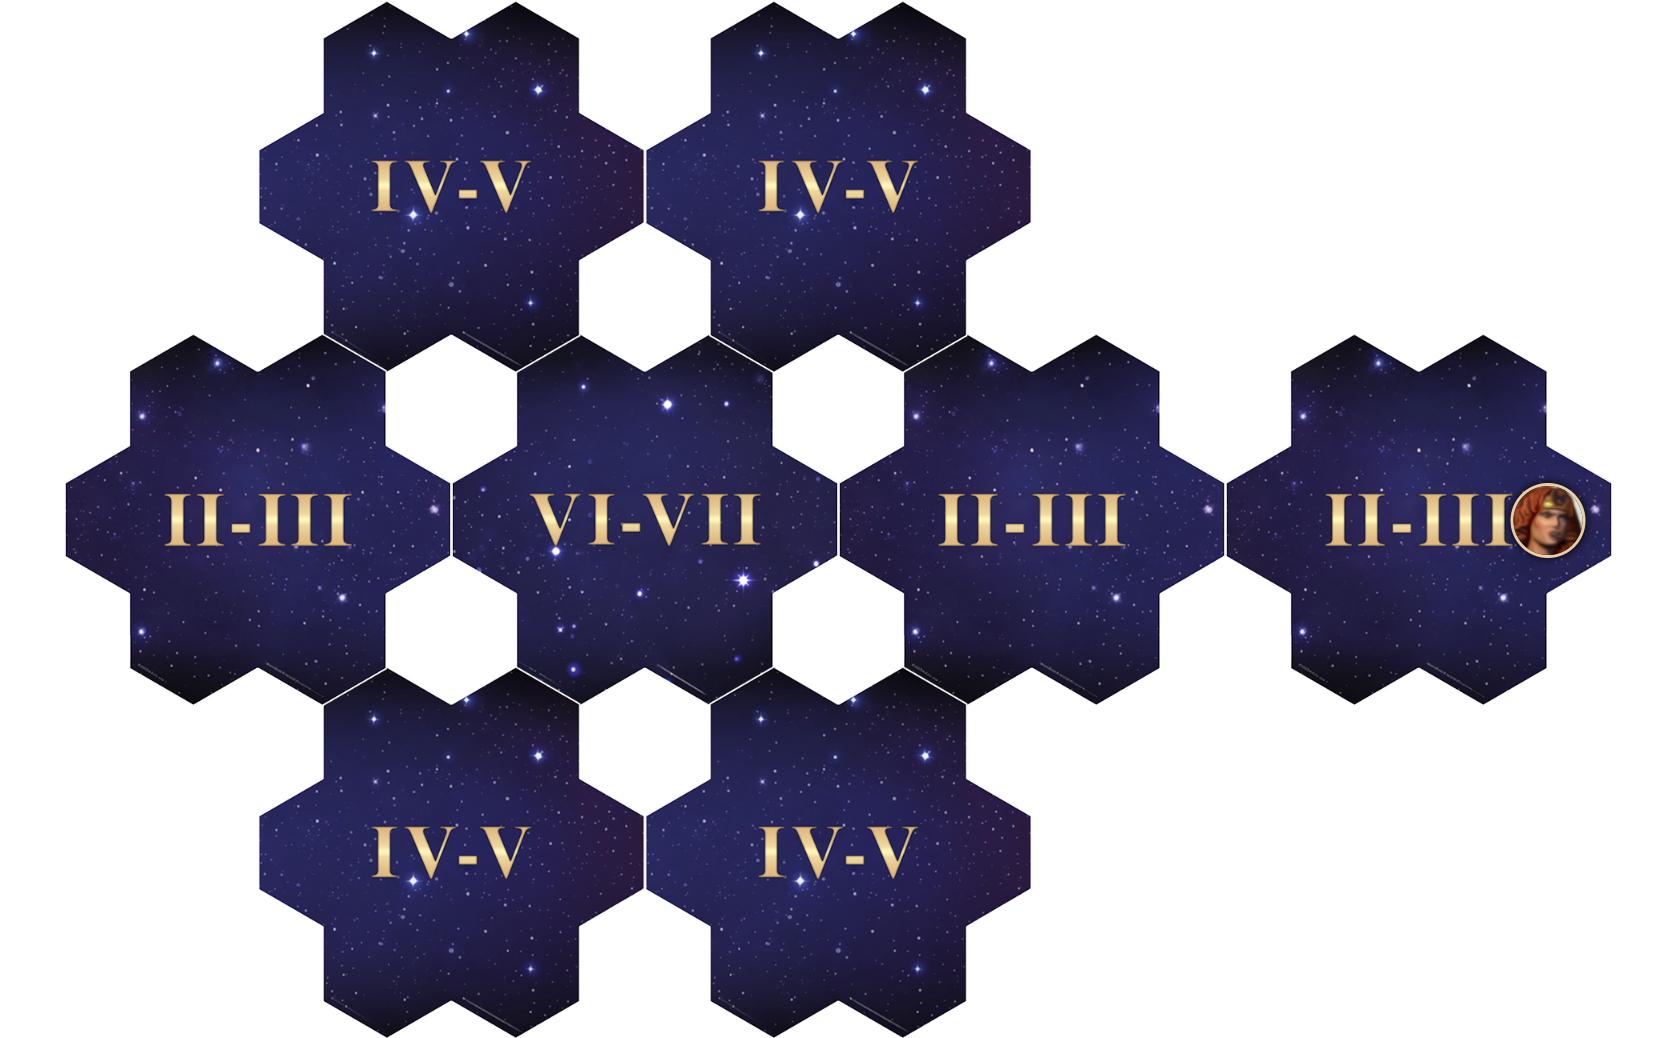
\includegraphics[width=0.80\paperwidth]{\_assets/maps/castle_sicilian_dragon.png}
  };
\end{tikzpicture}

\newpage

\begin{multicols*}{2}

\subsection*{\MakeUppercase{The story}}

\textbf{Into the Badlands}

Catherine crossed arms and leaned on her saddle horn as she peered out over the wasteland they'd been led to.
The Archangels had gone ahead of the small force she'd scraped together, and she wondered if it had been a mistake to let them go.
With the enemy stronghold still nowhere in sight, locating it would take time, and the inhospitable landscape would not be kind.

Rion pulled up next to her as he finished gulping the last contents of a water pouch.
He wiped the dribble and sweat from his face before saying anything.
``Not the best place to do any fighting.
Besides the poor conditions, I've heard the locals are known for their particular… ferocity.''

``Well then, we'll just have to bring them to heel,'' Catherine replied coldly.
The truth was she was more worried about that possibility than she let on, but she had to maintain her composure to protect the image of her strength.

``You think they'll fight for us?'' Rion asked with a raised eyebrow.

Catherine tightly gripped a heavy sack of coin by her side and heaved it into her lap so the contents jingled like tiny bells to emphasize her point.
``I think generous arrangements can be made.
For the rest, the sword will do.''

\textbf{The First Relic}

Ahead, a clearing of dry, cracked ground gave way to a large Obelisk protruding from the ground like a massive marker.
Catherine had seen enough magical artifacts in her time that she could tell the structure was a place of power.
Throwing an arm forward, she signaled Rion to proceed with an inspection.

The mage approached slowly, removing a glove to touch the cold stone of the smoothly cut sides with his skin.
Intricate runes were carved in it, detailing all manner of scripture in long-lost tongues.
As awe-inspiring as it was, equally apparent was the time-worn damage.

After a moment, he turned to Catherine.
``It's a transport beacon,'' he said.
``Like a monolith, but with a shorter range.
At least… it was.
It's damaged, and where the magic in the runes should be strong, even glowing, they're dark, and any power is long decayed.''

Catherine dismounted and slowly inspected the area before saying anything.
``Some of the damage is recent.
I can still feel residual heat; the Archangels were here.''

``How can you be sure? Surely, some would have found us by now and notified us of their progress.''

``They've never let me down,'' Catherine grunted.
``Come, let's see if other such beacons exist.''

\textbf{Showdown}

Sounds of battle perked the ears of Catherine's forces, and she urged her steed forward to catch sight of the combatants.

Rounding crags and jagged rocks jutting at all angles, another Obelisk revealed itself with the final moments of a battle taking place around it.
Several Archangels were on the ground, locked in combat with the remains of a larger undead force.

Approaching at speed, Catherine raised a fist in the air to salute the holy warriors, and several rasped their bronze chestplates in return.

``Queen Catherine, you've saved us the trouble of finding you,'' the lead angel said in his deep voice.
He gestured to the Obelisk with an open palm as the sounds of battle finally died.
``The foes meant to keep us from these structures by destroying them.
We barely managed to intercept them in time to preserve this one.''

Rion trotted past them as they spoke, intent on inspecting the intact Obelisk.
As before, he began to place his hand on the cold stone, but recoiled before making contact.
``It's active!'' he said excitedly.
``This may be the break we need.
With luck, this will take us directly to the enemy stronghold.''

Catherine smiled, reaching to clasp the arm of the angel in thanks for his work.
She looked back at the ragtag group of forces she'd gathered and hoped it would be enough for a siege.

\begin{itemize}
  \item \textcolor{darkcandyapplered}{Add a Few Archangels to your army.}
  \item \textcolor{darkcandyapplered}{You may now teleport to the enemy town on Tile S1.
  If you choose not to, you may in the future by spending one movement at this Obelisk.}
\end{itemize}


\textbf{The Escape}

With the thick, macabre, almost demonic-looking walls breached and the bulk of the necromancer's forces slain, the castle belonged to Catherine.
It was an eye for an eye, and she relished driving the final blow into the last enemy ranks still in the courtyard herself.

Unfortunately, after a frantic search of the grounds, Vhidhax himself was nowhere in sight.
Catherine raced up the walls just in time to peer over the side and catch sight of the necromancer fleeing with a sizable retinue that had quietly slipped away during the battle.
He was traveling north, further into the badlands and away from her home.
Catherine's campaign wasn't finished yet.

Catherine turned to observe the battlefield from above.
The butcher's bill had been large.
Both fresh and long-decaying bodies lay strewn about, several Archangels among them.
Rion caught up with her a minute later, and the two exchanged looks of exhaustion.

``It's done,'' Rion said through panting breaths.

``No.
The necromancer lives, and he flees north.''

``But… our forces.
The Archangels are too few to continue; what hope do we have?''

``There is always hope, my friend.
We'll use this castle as a base to resupply, and then we need to give chase before the fiend regains his strength.
Steadwick will never be safe otherwise!''

``This is foolish,'' Rion sighed.
``We don't need to fight this hard; Vhidhax is not your father, Catherine…''

\begin{itemize}
  \item \textcolor{darkcandyapplered}{Remove Archangels from your army, if possible.}
  \item \textcolor{darkcandyapplered}{Keep the rest of your army and resources for the next Scenario.}
  \item \textcolor{darkcandyapplered}{Reset your Hero per the normal campaign rules.}
\end{itemize}

\vspace{2em}
\begin{center}
  \framedimage[0.75\linewidth]{\art/necropolis_town.jpg}
\end{center}

\end{multicols*}
